\section{Processing Data With QC\_PH}
\label{sec:QC_PH}

QC\_PH is a standalone Matlab program that reads data files from the \instType{} Client. This program does a better job of filtering out outlying blanks and sample points that resulted from air bubbles, and flags those points as well as points where a mechanical error such as a failed valve or pump might have occurred. pH values calculated from SAMI\_Client and QC\_PH will differ slightly, due to blank filtering an smoothing by QC\_PH.  QC\_PH provides more reliable pH values.

\subsection{Installing Matlab Runtime and QC\_PH Application}

On the \instType{} disk, open the folder \textbf{QC\_PH}, open the appropriate folder for Macintosh or PC, then double-click on the application.  This will guide you through installation of Matlab runtime as well as QC\_PH.  It will require web access and will take a bit of time, depending on the speed of the internet connection.  Future updates to QC\_PH will install quickly, once the runtime has been installed.  If you need a complete installer (no internet access), please contact technical support. The default folder for the application is Programs\textbackslash Sunburst Sensors\textbackslash. You can move an alias of the application to a more convenient location.  

\subsection{Running QC\_PH}
\label{sec:RunQC_PH}

\begin{wrapfigure}[18]{l}{0.6\textwidth}
\centering
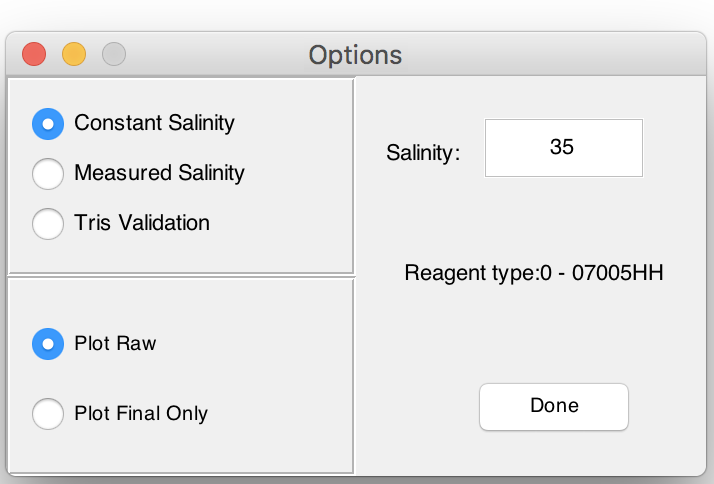
\includegraphics[width=0.9\textwidth]{figs/PH_Options.png}
\caption{PH Options.}
\label{fig:Options}
\end{wrapfigure}

To run QC\_PH, double click on the icon. You will be prompted to choose the \instType{} data file.  After reading the file, the app will ask you to choose \textbf{Constant Salinity}, \textbf{Measured Salinity}, or \textbf{Tris Validation}.  Choose \textbf{Constant Salinity} if salinity was not measured, but you know the approximate value.  Choose \textbf{Measured Salinity} if you have a data file from a CTD that was deployed with the \instType{} you will next be prompted to choose the CTD file.  This file must be a tab delimited text file in the format: dd/mm/yy Tab \normalfont {hh}$\colon$\normalfont {mm}$\colon$\normalfont {ss} Tab salinity.  Choose \textbf{Tris Validation} if you are running a Tris buffer with known pH for validation of instrument accuracy.

\begin{wrapfigure}[12]{r}{0.6\textwidth}
\centering
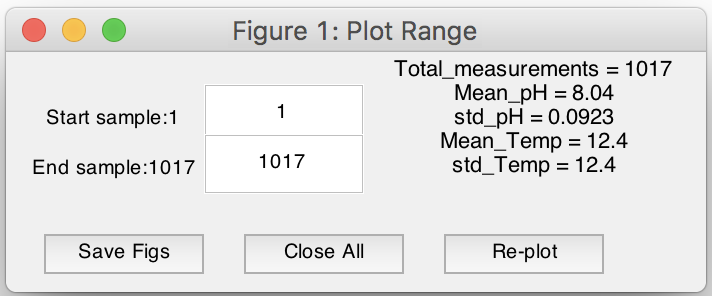
\includegraphics[width=0.9\textwidth]{figs/Plot_Range.png}
\caption{PH Options.}
\label{fig:Options}
\end{wrapfigure}

QC\_PH will calculate pH and shows plots of signals, absorbances, blanks, point pH, temperature, and final pH.  These plots can be useful in troubleshooting a \instType{}.  You can set the range of samples to view by changing the \textbf{Start Sample} and \textbf{End Sample} and selecting \textbf{Re-Plot} on Figure 1. Select \textbf{Save Figs} to save the figures and \textbf{Close All} to close the Figure windows.  Figures and a text file of the output data will be saved in a folder named \say{Filename\_Results.}

\subsection{Interpreting QC\_PH Data and Figures}
QC\_PH will plot several figures.  The figures that are often used to determine data quality and instrument performance are described here.  

The \textbf{Intensity/Absorbance} plot indicates instrument performance (Figure \ref{fig:Blanks}).  The top plot is reference signals, which should remain constant, but might degrade gradually over the course of a deployment.  The middle plot is signals through the optical cell.  These signals start high at the beginning of a sample, drop as indicator moves through the cell, and gradually increase.  Smooth curves indicate the \instType{} is working well, whereas flat lines or many spikes in signals indicates malfunction. The signals are plotted \say{Raw} and after outlying points are filtered out.

The \textbf{Blank} plot plots the signals of the blanks measured at the beginning of each sample (Figure \ref{fig:Blanks}).  These signals will degrade gradually over the course of a deployment, but should not have large spikes, and should remain above \ifcase \inst {7000.} \else {1000.} \fi

\begin{figure}[!h]
\begin{minipage}[t]{0.45\textwidth}
\centering
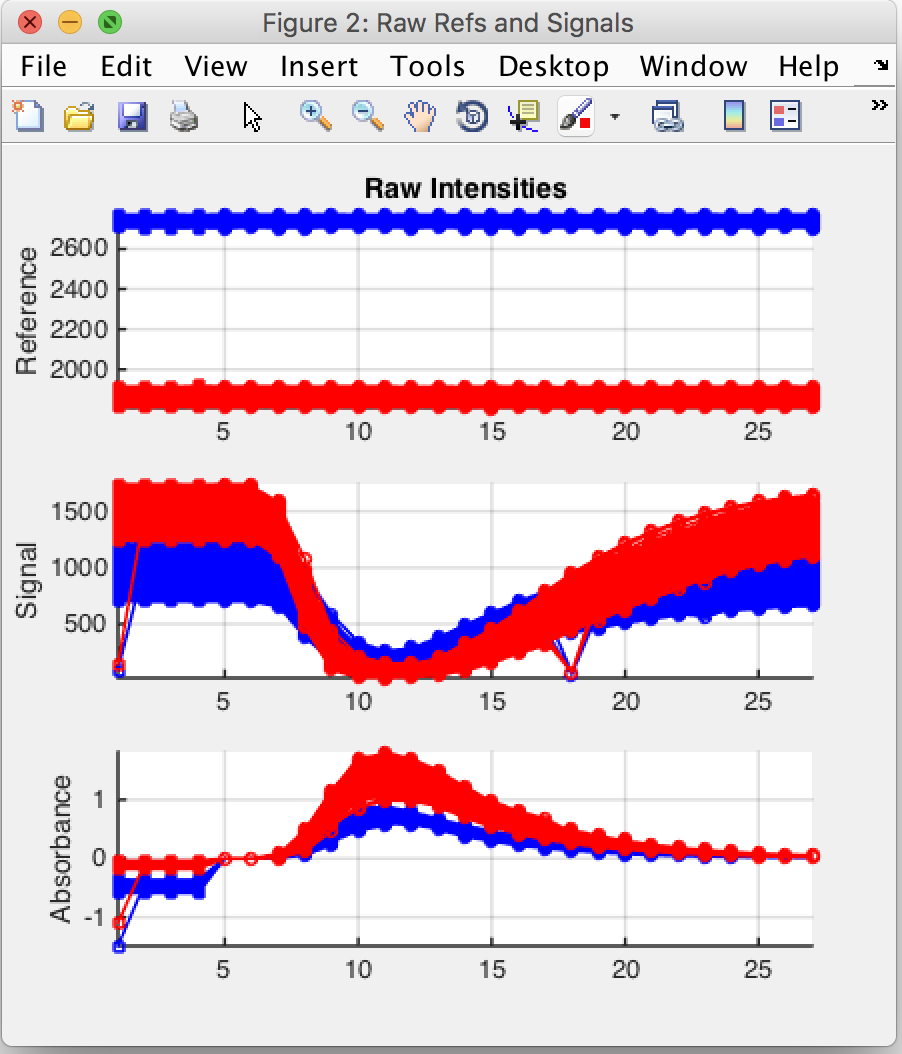
\includegraphics[width=0.9\textwidth]{figs/Intensities.png}
\end{minipage}

\begin{minipage}[t]{0.45\textwidth}
\centering
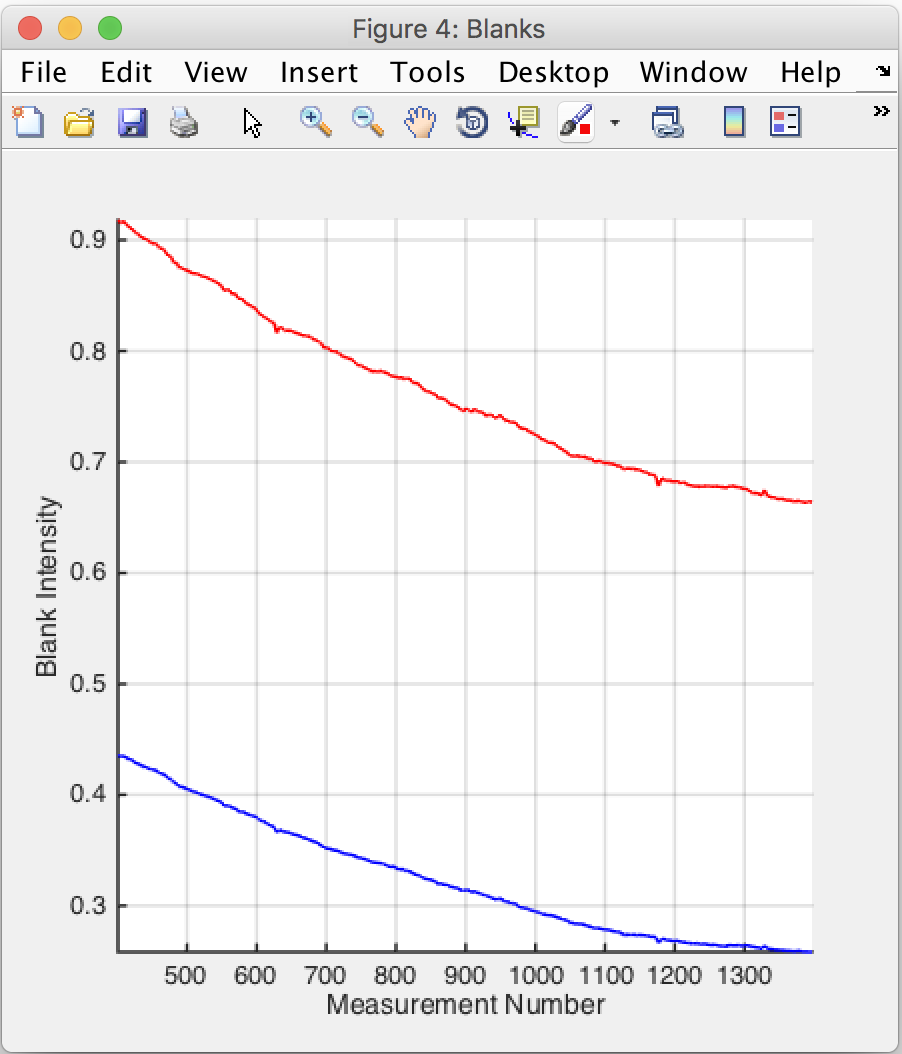
\includegraphics[width=0.9\textwidth]{figs/Blanks.png}
\end{minipage}

\captionof{figure}{Signal intensity plots (left) are plotted as 28 points for each measurement (top: reference signals, middle: signals through cell, bottom: absorbances through cell); ratios of blank signal/reference signal (right) are plotted as one point per measurement. 434\,nm signal shown in blue; 578\,nm signal shown in red.}
\label{fig:Blanks}
\end{figure}

The \textbf{Final pH} plot shows the temperature and pH measured throughout the deployment (Figure \ref{fig:FinalpH}).  pH noise from one measurement to another should be less than 0.002\,pH and temperature noise should be less than 0.05\,$\degree$C.  As blank signals degrade, pH precision might also degrade.

\begin{figure}
\centering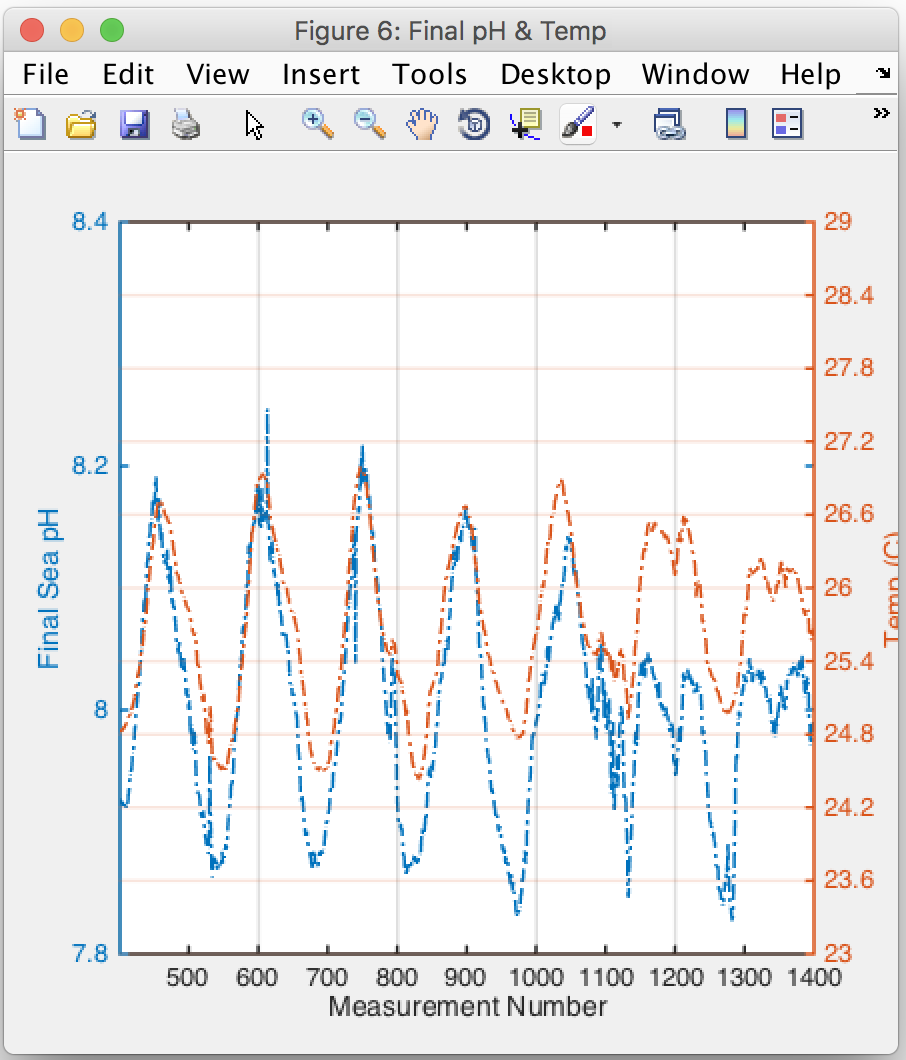
\includegraphics[width=0.6\textwidth]{figs/Final_PH.png}
\caption{Final pH (blue) and Temperatue (orange).}
\label{fig:FinalpH}
\end{figure}